\documentclass[10pt,mathserif]{beamer}
\usepackage[english]{babel}
\usepackage[utf8]{inputenc}
\usepackage[T1]{fontenc}
\usepackage{cmbright}
\usepackage{tikz}
\usepackage{listings}
\usepackage{relsize}

\usetikzlibrary{arrows}
\usetikzlibrary{backgrounds}
\usetikzlibrary{chains}
\usetikzlibrary{fit}
\usetikzlibrary{positioning}
\usetikzlibrary{scopes}
\usetikzlibrary{trees}

\usetheme{Warsaw}
\useoutertheme{essential}
\setbeamertemplate{navigation symbols}{}

\author{Stefano Cherubin}
\institute{Politecnico di Milano}
\date{06-05-2016}
\title{Introduction to LLVM compiler framework}
\newcommand{\customdata}{Stefano Cherubin <stefano.cherubin@polimi.it>}
\renewcommand{\ttdefault}{pxtt}
\lstset{basicstyle=\ttfamily\scriptsize}
\newcommand{\cinput}[1]{\lstinputlisting[language=C]{#1}}
\newcommand{\cinline}[1]{\lstinline[language=C]!#1!}
\newcommand{\llvminput}[1]{\lstinputlisting[language=LLVM]{#1}}
\newcommand{\llvminline}[1]{\lstinline[language=LLVM]!#1!}
\lstdefinelanguage{LLVM}%
  {morekeywords={define,declare,global,constant,internal,external,private,%
      linkonce,linkonce_odr,weak,weak_odr,appending,common,extern_weak,%
      thread_local,dllimport,dllexport,hidden,protected,default,except,deplibs,%
      volatile,fastcc,coldcc,cc,ccc,x86_stdcallcc,x86_fastcallcc,ptx_kernel,%
      ptx_device,signext,zeroext,inreg,sret,nounwind,noreturn,nocapture,byval,%
      nest,readnone,readonly,noalias,uwtable,inlinehint,noinline,alwaysinline,%
      optsize,ssp,sspreq,noredzone,noimplicitfloat,naked,alignstack,module,asm,%
      align,tail,to,addrspace,section,alias,sideeffect,c,gc,target,datalayout,%
      triple,blockaddress},%
  morekeywords=[2]{add,fadd,sub,fsub,mul,fmul,sdiv,udiv,fdiv,srem,urem,frem,%
     and,or,xor,icmp,fcmp,eq,ne,ugt,uge,ult,ule,sgt,sge,slt,sle,oeq,ogt,oge,%
     olt,ole,one,ord,ueq,ugt,uge,ult,ule,une,uno,nuw,nsw,exact,inbounds,phi,%
     call,select,shl,lshr,ashr,va_arg,trunc,zext,sext,fptrunc,fpext,fptoui,%
     fptosi,uitofp,sitofp,ptrtoint,inttoptr,bitcast,ret,br,indirectbr,switch,%
     invoke,unwind,unreachable,malloc,alloca,free,load,store,getelementptr,%
     extractelement,insertelement,shufflevector,extractvalue,insertvalue},%
  sensitive=t,%
  morestring=[b]",%
  morecomment=[l];%
  }[keywords,comments,strings]

\AtBeginSection[]
{
\begin{frame}{Contents}
\tableofcontents[currentsection]
\end{frame}
}
\begin{document}

\begin{frame}
\maketitle
\begin{center}
\itshape\scriptsize This material is strongly based on material produced by
                    Michele Scandale and Ettore Speziale for the course
                    `Code Optimizations and Transformations`.
\end{center}
\end{frame}

\section{Introduction}
\begin{frame}{Compilers and compilers}
Approaching to compilers, we need to understand the difference between a
\emph{toy-compiler} and \emph{production-quality compiler}.
\begin{columns}[t]
\column{.40\textwidth}
\begin{block}{Toy Compiler}
\begin{itemize}
\item small code-base
\item easy doing tiny edits
\item impossible doing normal/big edits
\end{itemize}
\end{block}

\column{.50\textwidth}
\begin{block}{Production-Quality Compiler}
\begin{itemize}
\item huge code-base
\item difficult performing any kind of edits
\item compiler-code extremely optimized
\end{itemize}
\end{block}
\end{columns}

\vfill
Key concepts:

\begin{itemize}
\item working with a production-quality compiler is \emph{initially} \alert{hard},
      but \ldots
\item \ldots an huge set of tools for analyzing/transforming/testing code
      is provided -- toy compilers \alert{miss these things}!
\end{itemize}
\end{frame}

\begin{frame}{LLVM: Low Level Virtual Machine}
Initially started as a research project at Urbana-Champaign:

\begin{itemize}
\item now intensively used for \alert{researches} involving compilers
\item key technology for \alert{leading industries} -- AMD, Apple, Intel,
      NVIDIA
\end{itemize}

\vfill
If you are there, then it is \alert{your key-technology}:

\begin{itemize}
\item open-source compilers: Open64~\cite{LOCAL:www/open64},
      GCC~\cite{LOCAL:www/gcc}, LLVM~\cite{LOCAL:www/llvm}
\item LLVM is relatively \alert{young} -- GCC performances are  better -- but \ldots
\item \ldots it is highly modular, well written, kept \emph{clean} by developers.
\end{itemize}
\end{frame}

\section{Compiler organization}
\begin{frame}{Compiler pipeline}
Tipically a compiler is a \alert{pipeline}:

\begin{figure}
\centering

% compiler-structure.tex: generic organization of a compiler.

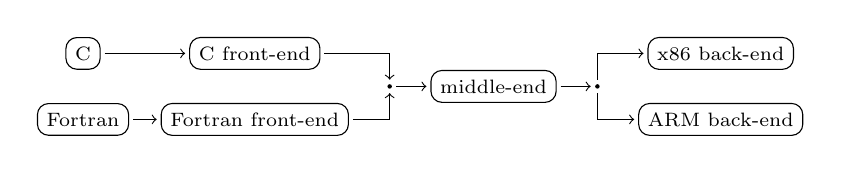
\begin{tikzpicture}
[
  every node/.style={
    font=\scriptsize
  },
  cell/.style={
    rectangle,
    rounded corners,
    draw
  },
  point/.style={
    circle,
    fill,
    inner sep=.2mm
  },
  tip/.style={
    ->,
    shorten >=.5mm,
    shorten <=.5mm
  },
  man-tip/.style={
    tip,
    to path={-| (\tikztotarget)}
  },
  rman-tip/.style={
    tip,
    to path={|- (\tikztotarget)}
  }
]

\matrix [column sep=4mm]
{
\node (c-language)   [cell] {C};             &
\node (c-front-end)  [cell] {C front-end};   &
\node ()             []     {};              &
\node ()             []     {};              &
\node ()             []     {};              &
\node (x86-back-end) [cell] {x86 back-end}; \\

\node ()               []      {};           &
\node ()               []      {};           &
\node (middle-end-in)  [point] {};           &
\node (middle-end)     [cell]  {middle-end}; &
\node (middle-end-out) [point] {};           &
\node ()               []      {};          \\

\node (fortran-language)  [cell] {Fortran};           &
\node (fortran-front-end) [cell] {Fortran front-end}; &
\node ()                  []     {};                  &
\node ()                  []     {};                  &
\node ()                  []     {};                  &
\node (arm-back-end)      [cell] {ARM back-end};     \\
};

{ [start chain]
\chainin (c-language)    [join];
\chainin (c-front-end)   [join=by tip];
\chainin (middle-end-in) [join=by man-tip];
}

{ [start chain]
\chainin (fortran-language)  [join];
\chainin (fortran-front-end) [join=by tip];
\chainin (middle-end-in)     [join=by man-tip];
}

{ [start chain]
\chainin (middle-end-in)  [join];
\chainin (middle-end)     [join=by tip];
\chainin (middle-end-out) [join=by tip];
}

{ [start chain]
\chainin (middle-end-out) [join];
\chainin (x86-back-end)   [join=by rman-tip];
}

{ [start chain]
\chainin (middle-end-out) [join];
\chainin (arm-back-end)   [join=by rman-tip];
}
\end{tikzpicture}

\end{figure}

\vfill
There are three main components:
\begin{description}
\item[Front-end] \alert{translate} a source file in the \alert{intermediate representation}
\item[Middle-end] \alert{analyze} intermediate representation, \alert{optimize}
                  it
\item[Back-end] \alert{generate} target machine assembly from the interemediate
                representation
\end{description}
\end{frame}

\begin{frame}{Compiler pipeline}{Internal pipelines}
Each component is composed internally by pipelines:

\begin{itemize}
\item simple model of computations -- \alert{read} something, \alert{produce}
      something
\item only needed to specify \alert{how to transform} input data into output
      data
\end{itemize}

Complexity lies on \alert{chaining} together stages.
\end{frame}

\begin{frame}{Compiler pipeline}
We will consider only the \emph{middle-end}: same concepts are
valid also for \{front,back\}-end.

\vfill
Technical terms:
\begin{description}
\item[Pass] a pipeline stage
\item[IR] (a.k.a. Intermediate Representation) is the language used in the
          middle-end.
\end{description}

\vfill
The \alert{pass manager} manages a set of passes:
\begin{itemize}
\item build the compilation pipeline: \alert{schedule} passes together
      according to \alert{dependencies}.
\end{itemize}

\vfill
Dependencies are \alert{hints} used by the pass manager in order to schedule passes.
\end{frame}

\begin{frame}{First insights}
A compiler is \alert{complex}:

\begin{itemize}
\item passes are the \alert{elementary unit of work}
\item pass manager must be \alert{advisee} about pass chaining
\item pipeline shapes are \alert{not fixed} -- it can change from one compiler
      execution to another~\footnote{e.g. optimized/not optimized builds}
\end{itemize}

\vfill
Moreover, compilers must be \alert{conservative}:

\begin{itemize}
\item apply a transformation only if program \alert{semantic is preserved}
\end{itemize}

\vfill
Compiler algorithms are designed differently!
\end{frame}

\section{Algorithm design}
\begin{frame}{Classical Algorithm Design}
Dealing with algorithm design, a good approach is the following:
\begin{enumerate}
\item study the problem
\item make some example
\item identify the \alert{common case}
\item derive the algorithm for the common case
\item add handling for \alert{corner cases}
\item improve performancing \alert{optimizing the common case}
\end{enumerate}

\vfill
Weakness of the approach:
\begin{itemize}
\item \alert{corner cases} -- a \emph{correct} algorithm \textbf{must} consider \emph{all the corner cases}!
\end{itemize}
\end{frame}

\begin{frame}{Compiler Algorithm Design}{Be Conservative}
Corner cases are difficult to handle:

\begin{itemize}
\item compiler algorithms must be \alert{proved} to preserve program semantic
\item having a common methodology helps on that
\end{itemize}
\vfill
Compiler algorithms are built combining three kind of \alert{passes}:

\begin{itemize}
\item analysis
\item optimization
\item normalization
\end{itemize}

\vfill
We now consider a simple example: \emph{loop hoisting}.
\end{frame}

\begin{frame}{Loop Hoisting}
It is a transformation that:
\begin{itemize}
\item looks for statements (inside the loop) not depending on the loop state
\item move them outside the loop body
\end{itemize}

\begin{columns}[t]
\column{.45\textwidth}
\begin{block}{Loop Hoisting -- Before}
\centering
\cinput{snippet/01/loop-hoisting-before.c}
\end{block}

\column{.45\textwidth}
\begin{block}{Loop Hoisting -- After}
\centering
\cinput{snippet/01/loop-hoisting-after.c}
\end{block}
\end{columns}
\end{frame}


\begin{frame}{Loop Hoisting}{Focus on the Transformation}
The transformation is trivial:

\begin{itemize}
\item move ``good'' statement outside of the loop
\end{itemize}

This is the \alert{optimization pass}. It needs to known:

\begin{itemize}
\item loops
\item ``good'' statements
\end{itemize}

They are \alert{analysis} passes:

\begin{itemize}
\item detecting loops in the program
\item detecting loop-independent statements
\end{itemize}

When registering loop hoisting, also declare needed analysis:

\begin{itemize}
\item pipeline automatically built -- analysis $\rightarrow$ optimization
\end{itemize}
\end{frame}

\begin{frame}{Loop Hoisting}{Proving Program Semantic Preservation}
The proof is trivial:

\begin{itemize}
\item transformation is correct if analysis are correct, but \ldots
\item \ldots usually analysis are built starting from other analysis already
      implemented inside the compiler
\end{itemize}

You have to prove that combining all analysis information gives you a
correct view of the code:

\begin{itemize}
\item analysis information cannot induce optimization passes applying a
      transformation not preserving program semantic
\end{itemize}
\end{frame}

\begin{frame}{Loop Hoisting}{More Loops}
We have spoken about loops, but which kind of loop?

\begin{itemize}
\item \cinline{do-while} loops?
\item \cinline{while} loop?
\item \cinline{for} loops?
\end{itemize}

We have seen loop hoisting on:

\begin{itemize}
\item \cinline{do-while} loops
\end{itemize}

What about other kinds of loops?

\begin{itemize}
\item they must be normalized -- i.e. transformed to \cinline{do-while} loops
\end{itemize}

\alert{Normalization passes} do that:

\begin{itemize}
\item before running loop hoisting, you must tell to the pass manager that loop
      normalization must be run before
\end{itemize}

This allows to recognize more loops, thus potentially improving optimization
impact!
\end{frame}

\begin{frame}{Compiler Algorithm Design}{A methodology}
You have to:

\begin{enumerate}
\item analyze the problem
\item make some examples
\item detect the common case
\item declare the \alert{input format}
\item declare \alert{analysis} you need
\item design an \alert{optimization} pass
\item proof its \alert{correctness}
\item improve algorithm perfomance by acting on common case -- the only
      considered up to now. Please notice that corner cases are not considered
      -- just do not optimize
\item improve the effectiveness of the algorithm by adding
      \alert{normalization passes}
\end{enumerate}
\end{frame}

\section{Inside LLVM}
\begin{frame}{Terminology}{Speaking About LLVM IR}
LLVM IR comes with 3 different flavours:

\begin{description}
\item[assembly] human-readable format
\item[bitcode] binary on-disk machine-oriented format
\item[in-memory] binary in-memory format, used during compilation process
\end{description}

All formats have the same expressiveness!

\bigskip
File extensions:

\begin{description}
\item[.ll] for assembly files
\item[.bc] for bitcode files
\end{description}
\end{frame}

\begin{frame}{Tools}{C Language Family Front-end}
Writing LLVM assembly by hand is unfeasible:

\begin{itemize}
\item different front-ends available for LLVM
\item use Clang~\cite{LOCAL:www/clang} for the C family
\end{itemize}

The clang driver is compatible with GCC:

\begin{itemize}
\item $\approx$ same command line options
\end{itemize}

To generate LLVM IR:

\begin{description}
\item[assembly] \texttt{\smaller clang -emit-llvm -S -o out.ll in.c}
\item[bitcode] \texttt{\smaller  clang -emit-llvm -o out.bc in.c}
\end{description}

It can also generate native code starting from LLVM assembly or LLVM bitcode --
like compiling an assembly file with GCC
\end{frame}

\begin{frame}{Tools}{Playing with LLVM Passes}
LLVM IR can be manipulated using \texttt{\smaller opt}:

\begin{itemize}
\item read an input file
\item run specified LLVM passes on it
\item respecting user-provided order
\end{itemize}

Useful passes:

\begin{itemize}
\item print CFG with \texttt{\smaller opt -view-cfg input.ll}
\item print dominator tree with \texttt{\smaller opt -view-dom input.ll}
\item \ldots
\end{itemize}

Pass chaining:

\begin{itemize}
\item run \emph{mem2reg}~\footnote{More on this later}, then view the CFG with
      \texttt{\smaller opt -mem2reg -view-cfg input.ll}
\end{itemize}
\end{frame}

\begin{frame}{Pass Hierarchy}
LLVM provides a lot of passes:

\begin{itemize}
\item try \texttt{\smaller opt -help}
\end{itemize}

For performance reasons there are different kind of passes:

\begin{block}{LLVM Passes}

% llvm-passes: hierarchy of LLVM passes.

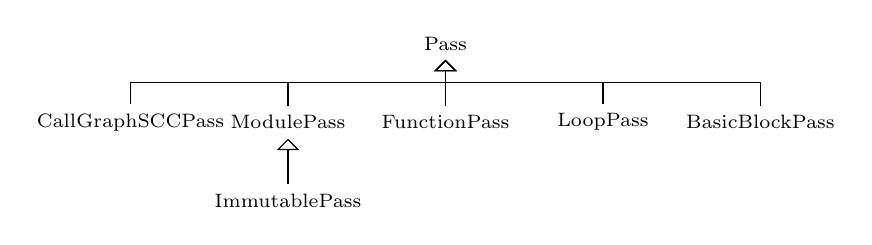
\begin{tikzpicture}
[
  every node/.style={
    font=\scriptsize
  },
  extends/.style={
    draw,
    open triangle 90-
  },
  level distance=10mm,
  level 1/.style={
    sibling distance=20mm
  },
  level 3/.style={
    sibling distance=20mm
  }
]

\node {Pass}
  [edge from parent fork down,
   edge from parent/.style={extends}]

  child { node {CallGraphSCCPass}}
  child { node {ModulePass}
    child { node {ImmutablePass}}
  }
  child { node {FunctionPass}}
  child {node {LoopPass}}
  child {node {BasicBlockPass}};
\end{tikzpicture}

\centering
\end{block}
\end{frame}

\begin{frame}{LLVM Passes}
Each pass kind visits particular elements of a module:

\begin{description}
\item[ImmutablePass] compiler configuration -- never run
\item[CallGraphSCCPass] post-order visit of CallGraph SCCs
\item[ModulePass] visit the whole module
\item[FunctionPass] visit functions
\item[LoopPass] post-order visit of loop nests
\item[BasicBlockPass] visit basic blocks
\end{description}

Specializations comes with restrictions:

\begin{itemize}
\item e.g. a \alert{FunctionPass} cannot add or delete functions
\item refer to~\cite{LOCAL:www/llvmWritingAPass} for accurate description of
      features and limitations of each kind of pass
\end{itemize}
\end{frame}

% \begin{frame}{Examples}
% Now we will see very simple passes:
%
% \begin{itemize}
% \item some of them are meaningless
% \item goal is to show you the LLVM API
% \end{itemize}
%
% \vfill
%
% The passes are:
% \begin{description}
% \item[instruction-count] simple instruction counting analysis
% \item[hello-llvm] optimization pass building an hello-world program
% \item[function-eraser] optimization pass removing ``small'' functions
% \end{description}
%
% \vfill
% Hint: take the LLVM pass writing tutorial~\cite{LOCAL:www/llvmWritingAPass}
% \end{frame}

\begin{frame}{What is Available Inside LLVM?}
LLVM provides passes performing basic transformations:

\begin{itemize}
\item variables promotion
\item loops canonicalization
\item \ldots
\end{itemize}

They can be used to \alert{normalize/canonicalize} the input:

\begin{itemize}
\item transform into a form analyzable for further passes
\end{itemize}

Input normalization is \alert{essential}:

\begin{itemize}
\item keep passes implementation manageable
\end{itemize}
\end{frame}

\section{LLVM-IR language}
\begin{frame}{LLVM IR}
LLVM IR~\cite{LOCAL:www/llvmLanguageRef} language is RISC-based:

\begin{itemize}
\item instructions operates on \alert{variables}~\footnote{Virtual registers}
\item only \llvminline{load} and \llvminline{store} access memory
\item \llvminline{alloca} used to reserve memory on function stacks
\end{itemize}
\vfill
There are also few \alert{high level instructions}:
\begin{itemize}
\item function call -- \llvminline{call}
\item pointer arithmetics -- \llvminline{getelementptr}
\item \ldots
\end{itemize}
\end{frame}

\begin{frame}{LLVM IR}{Types \& Variables}
LLVM IR is \alert{strongly typed}:

\begin{itemize}
\item e.g. you cannot assign a floating point value to an integer variable
without an explicit cast
\end{itemize}

\alert{Almost everything} is \alert{typed} -- e.g.:

\begin{description}
\item[functions] \llvminline{@fact} -- \llvminline{i32 (i32)}
\item[statements] \llvminline{\%3 = icmp eq i32 \%2, 0} -- \llvminline{i1}
\end{description}

A variable can be:

\begin{description}
\item[global] \llvminline{@var = common global i32 0, align 4}
\item[function parameter] \llvminline{define i32 @fact(i32 \%n)}
\item[local] \llvminline{\%2 = load i32, i32* \%1, align 4}
\end{description}

Local variables are defined by statements
\end{frame}

\begin{frame}{LLVM IR}{Example: factorial}

\begin{center}
\llvminput{snippet/01/fact.ll}
\end{center}
\end{frame}

\begin{frame}{LLVM IR Language}{Static Single Assignment}
LLVM IR is SSA-based:

\begin{itemize}
\item every variable is \alert{statically assigned} exactly \alert{once}
\end{itemize}

Statically means that:

\begin{itemize}
\item inside each function
\item for each variable \llvminline{\%foo}
\item there is only one statement in the form \llvminline{\%foo = ...}
\end{itemize}

Static is different from dynamic:

\begin{itemize}
\item a static assignment can be executed more than once
\end{itemize}
\end{frame}

\begin{frame}{Static Single Assignment}{Examples}
\begin{block}{Scalar SAXPY}
\centering
\cinput{snippet/02/scalar-saxpy.c}
\end{block}

\begin{block}{Scalar LLVM SAXPY}
\centering
\llvminput{snippet/02/scalar-saxpy.ll}
\end{block}

Temporary \llvminline{\%1} not reused! \llvminline{\%2} is used for the second
assignment!
\end{frame}

\begin{frame}{Static Single Assignment}{Examples}
\begin{block}{Array SAXPY}
\centering
\cinput{snippet/02/array-saxpy.c}
\end{block}

\begin{block}{Array LLVM SAXPY}
\centering
\llvminput{snippet/02/array-saxpy.ll}
\end{block}

One assignment for loop counter \llvminline{\%i.0}
\end{frame}

\begin{frame}{Static Single Assignment}{Handling Multiple Assignments}
\begin{block}{Max}
\centering
\cinput{snippet/02/max.c}
\end{block}

\begin{block}{LLVM Max -- Bad}
\centering
\llvminput{snippet/02/bad-max.ll}
\end{block}

Why is it bad?
\end{frame}

\begin{frame}{Static Single Assignment}{Use \llvminline{phi} to Avoid Troubles}
The \llvminline{\%2} variable must be statically set once

\begin{block}{LLVM Max}
\centering
\llvminput{snippet/02/good-max.ll}
\end{block}

The \llvminline{phi} instruction is a \emph{conditional move}:

\begin{itemize}
\item it takes $(variable_i, label_i)$ pairs
\item if coming from predecessor identified by $label_i$, its value is $variable_i$
\end{itemize}
\end{frame}

\begin{frame}{Static Single Assignment}{Definition and Uses}
Each SSA variable is set only once:

\begin{itemize}
\item variable \alert{definition}
\end{itemize}

Each SSA variable can be used by multiple instructions:

\begin{itemize}
\item variable \alert{uses}
\end{itemize}

Algorithms and technical language abuse of these terms:

\bigskip
\emph{
Let \llvminline{\%foo} be a variable. If \llvminline{\%foo} definition has not
side-effects, and no uses, dead-code elimination can be efficiently performed
by erasing \llvminline{\%foo} definition from the CFG.
}
\end{frame}

\begin{frame}{Static Single Assignment}{Rationale}
Old compilers are not SSA-based:

\begin{itemize}
\item putting input into SSA-form is expensive
\item cost must be amortized
\end{itemize}

New compilers are SSA-based:

\begin{itemize}
\item SSA easier to work with
\item SSA-based analysis/optimizations faster
\end{itemize}

All modern compilers are SSA-based:

\begin{itemize}
\item exception are old version of the HotSpot Client compiler
\end{itemize}
\end{frame}

\section{Conclusions}
\begin{frame}{Conclusions}
LLVM is a \alert{production-quality} compiler:

\begin{itemize}
\item[$\Rightarrow$] impossible knowing all details
\end{itemize}

But:

\begin{itemize}
\item is well organized
\item if you known compilers theory is ``easy'' finding what you need inside sources
\end{itemize}

Please take into account C++:

\begin{itemize}
\item basic skills required
\end{itemize}
\end{frame}

\section{Bibliography}
\begin{frame}[allowframebreaks]{Bibliography}
\nocite{*}
\bibliographystyle{plain}
\bibliography{bibliography}
\end{frame}
\end{document}
